\documentclass[conference]{IEEEtran}
\usepackage{amsmath,amssymb}
\usepackage{booktabs}
\usepackage{graphicx}
\usepackage{multirow}
\usepackage{url}
\usepackage{xcolor}
\graphicspath{{figures/}}

\title{An Explainable AI Framework for Analysis of X-Ray Polarimetry Data from XPoSat}

\author{
\IEEEauthorblockN{Author One, Author Two, Author Three, and Author Four}
\IEEEauthorblockA{Department of [Department Name], [College/University]\\
[City, Country]\\
[corresponding-author email]}
}

\begin{document}
\maketitle

\begin{abstract}
The Polarimeter Instrument in X-rays (POLIX) aboard XPoSat produces heterogeneous Level-2 products that require observation-level synthesis before archive screening. This work examines 25 POLIX observations included in a frozen project archive, comprising 10 project-labelled source observations and 15 project-labelled blank-sky observations. Exposure, channel-distribution, source-azimuth, delivered-light-curve, and cross-detector summaries are compressed into a traceable 15-feature Matrix-C representation. Standardization, principal component analysis, KMeans clustering, and Isolation Forest provide complementary views of this archive, with the fixed model artifact flagging four observations as anomaly candidates. A deterministic, project-specific local feature-ranking heuristic connects composite unusualness evidence to Matrix-C features and their product families. Seed, contamination, jackknife, feature-tier, and six-case neutralization analyses are treated as sensitivity or sanity checks rather than external validation. WeightedRoll is excluded from Matrix C and analysed independently through a weighted second-harmonic fit and an empirical reference formed from 13 qualifying blank-sky fits. Representative observations show that Matrix-C unusualness and modulation-like harmonic behaviour do not identify the same property within the project archive. The Flask interface exposes the saved workflow as a researcher-facing inspection prototype. The study is limited by the small unlabeled sample, archive-specific fitting, proxy feature semantics, source-plus-background WeightedRoll products, and absence of official background, polarization-degree, and sky-angle calibration.
\end{abstract}

\begin{IEEEkeywords}
XPoSat, POLIX, X-ray polarimetry, unsupervised anomaly detection, explainable artificial intelligence, scientific machine learning
\end{IEEEkeywords}

\section{Introduction}
X-ray polarimetry provides information complementary to timing, imaging, and spectroscopy by measuring the orientation dependence of detected radiation. XPoSat is an Indian Space Research Organisation (ISRO) mission carrying the Polarimeter Instrument in X-rays (POLIX) and the X-ray Spectroscopy and Timing instrument \cite{isro_xposat}. POLIX is a Thomson-scattering polarimeter, and its Level-2 release contains several observation products with different computational and physical meanings \cite{rishin2010thomson,fabiani2018instrumentation,polix_handbook_2025}. A researcher comparing observations must therefore reason across exposure, channel-distribution, source-azimuth, delivered-light-curve, detector, and roll-modulation products rather than analyse one homogeneous table.

This study treats this as an applied scientific-computing problem. It summarizes selected Level-2 products at observation level, screens the resulting vectors without trusted anomaly labels, ranks local feature evidence, and exposes the saved workflow through a Flask interface. Because trusted anomaly labels were unavailable, the final pipeline used a project-specific unsupervised explanation method rather than supervised or general post-hoc explainers.

WeightedRoll contains exposure-weighted source and background modulation contributions and is not assumed to be an officially background-corrected source product \cite{polix_handbook_2025}. It is excluded from the deployed feature matrix and fitted only in an independent harmonic branch. This prevents the same modulation information from generating an anomaly flag and then being used as circular confirmation.

Prior astronomical studies show the value of unsupervised ranking and human inspection in label-poor archives \cite{baron2017weirdest,giles2019serendipity,lochner2021astronomaly}. Explainable-anomaly work emphasizes that an explanation of unusualness is not the same as an explanation of a supervised label \cite{li2024explainable_anomaly}. Limited published work was identified that directly combines product-provenance-aware POLIX observation summaries, unsupervised screening of the project archive, local model-informed evidence ranking, and a separate blank-sky-referenced harmonic diagnostic. This is a scoped literature finding, not a priority or superiority claim.

The central question is whether heterogeneous POLIX Level-2 products can be represented through interpretable, product-aware features and screened using explainable unsupervised learning while maintaining an independent comparison with blank-sky-referenced harmonic modulation behaviour.

The primary contribution is a traceable, product-aware Explainable Artificial Intelligence (XAI) framework for screening heterogeneous POLIX Level-2 observations within the project archive. The secondary contributions are: (1) a 15-feature observation representation that preserves product-family provenance; (2) a deterministic, project-specific, model-informed local feature-ranking method; and (3) a scientifically separate WeightedRoll and empirical blank-sky harmonic branch. Robustness and neutralization analyses are sensitivity evidence, and the Flask interface is a reproducibility implementation rather than a separate major contribution.

\begin{figure}[t]
\centering
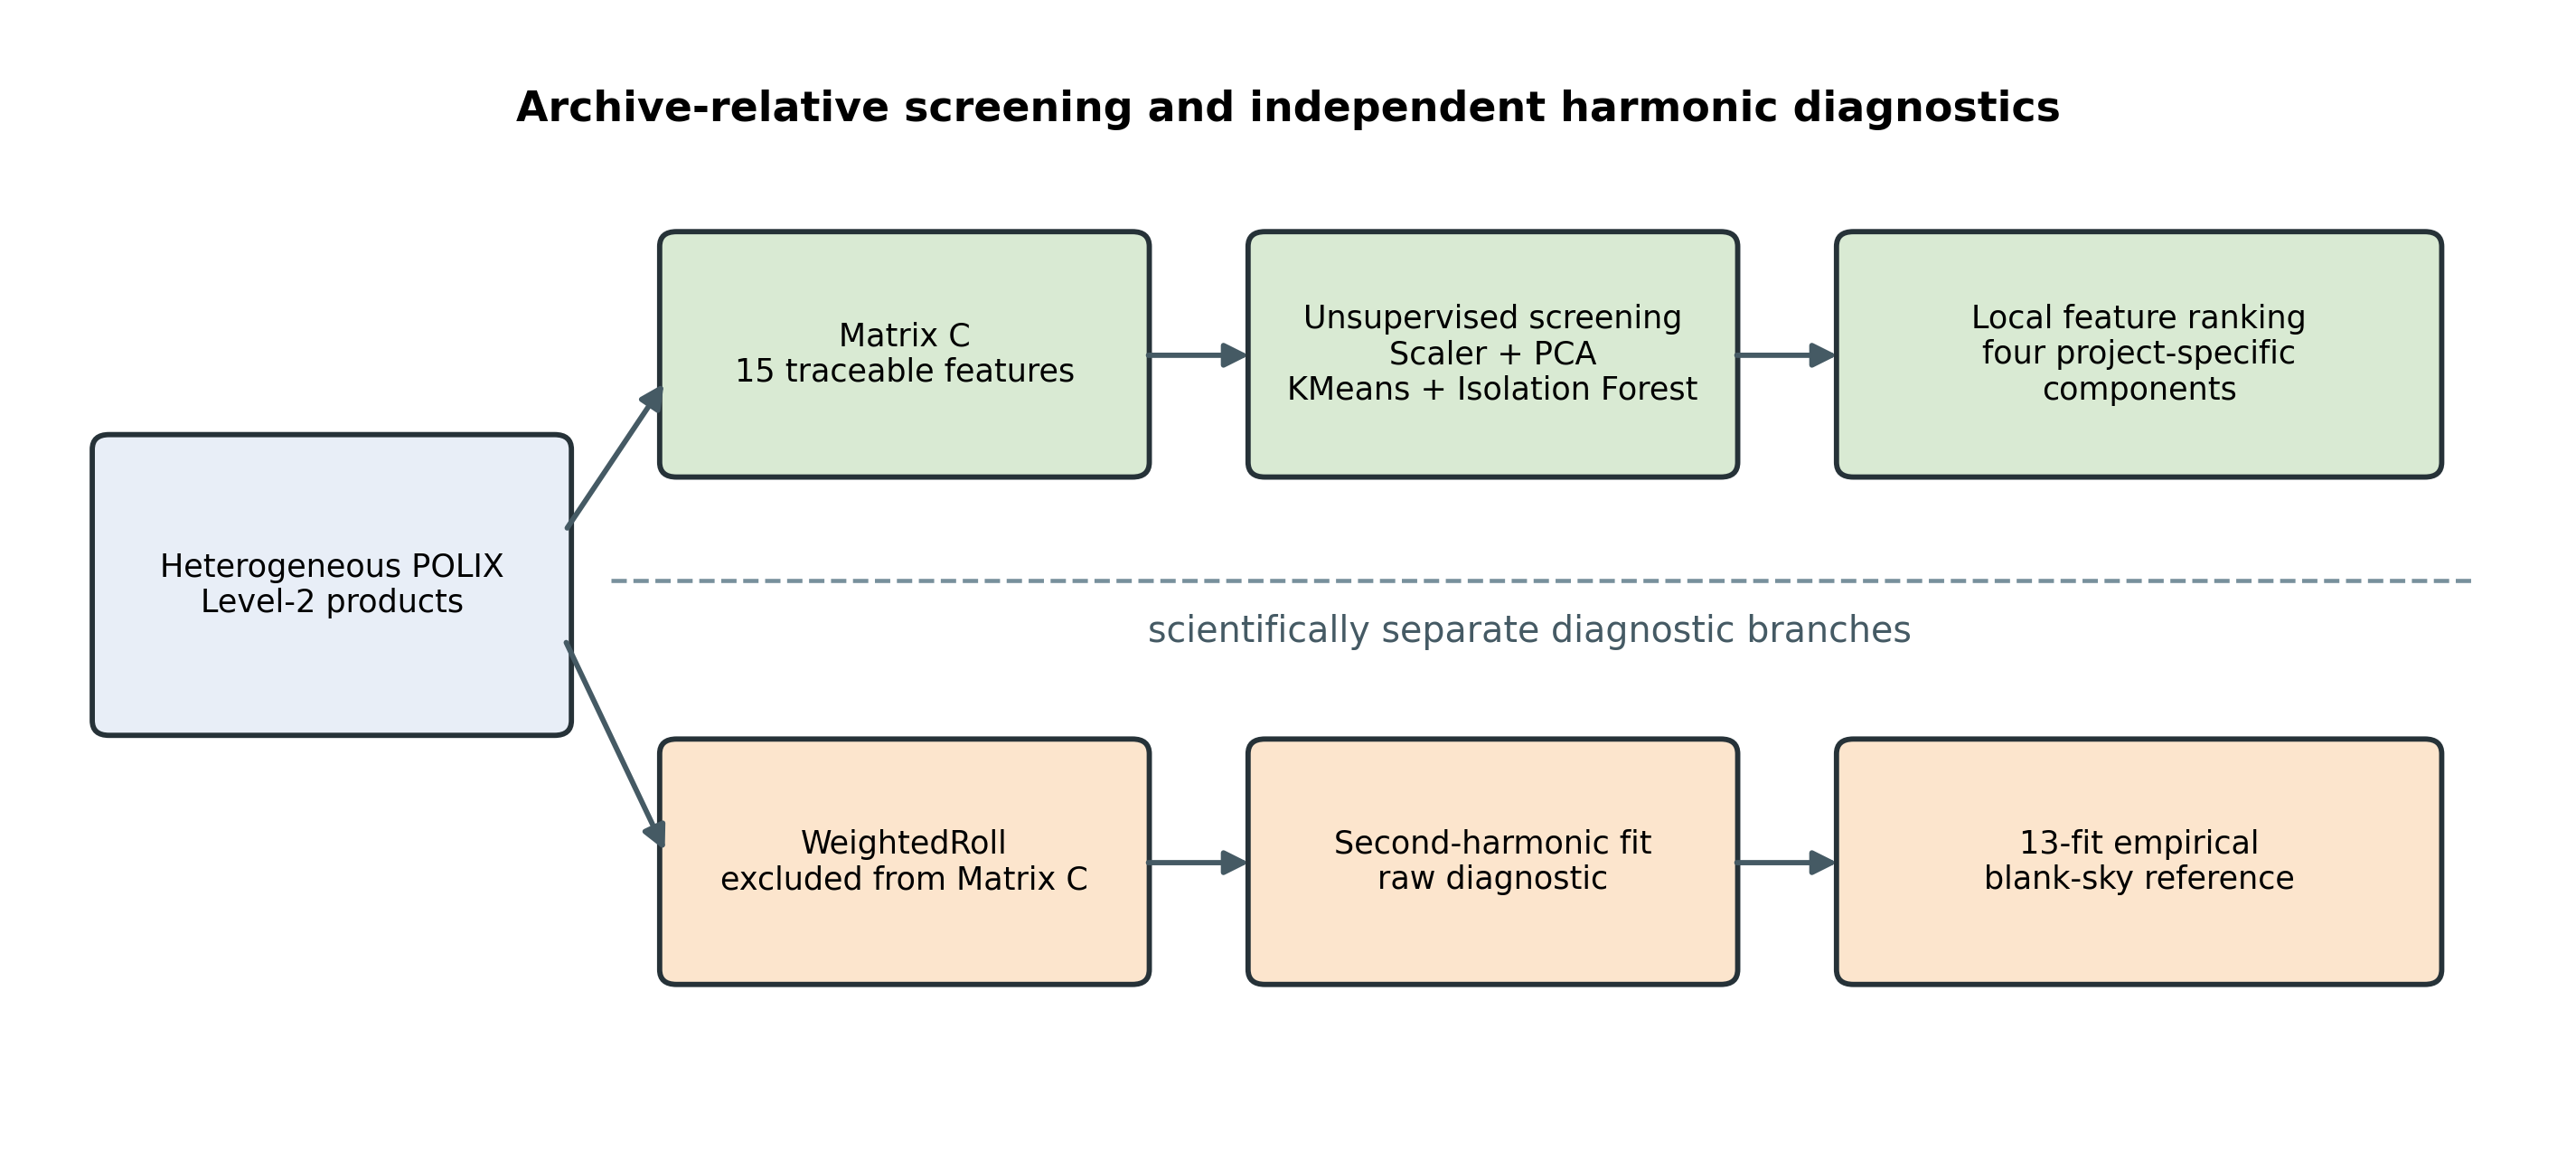
\includegraphics[width=\columnwidth]{fig1_framework_flow.png}
\caption{Framework flow. WeightedRoll is excluded from Matrix C and enters only the independent harmonic branch.}
\label{fig:framework}
\end{figure}

\section{Literature Review and Related Work}
\subsection{XPoSat, POLIX, and Polarimetric Analysis}
Official mission, archive, and handbook sources establish the mission scope, released-data organization, and product-use boundaries \cite{isro_xposat,issdc_xposat_archive,polix_handbook_2025}. POLIX measures azimuthal scattering behaviour associated with Thomson scattering \cite{rishin2010thomson}. Reviews describe how instrumental modulation, background, response calibration, and coordinate conventions enter physical polarization inference \cite{fabiani2018instrumentation}.

Linear cosine and sine coefficients provide a convenient second-harmonic representation, and Stokes-based treatments formalize related quantities \cite{kislat2015stokes}. Here the fitted values are called harmonic coefficients or fractional harmonic coordinates. They are not calibrated sky Stokes parameters because the project lacks an official background procedure, official modulation factor, and verified detector-to-sky angle conversion.

\subsection{Unsupervised Screening in Astronomy}
Principal component analysis (PCA), KMeans, and Isolation Forest provide complementary geometric, clustering, and isolation views \cite{pearson1901pca,macqueen1967kmeans,liu2008isolation}. The saved implementation uses their scikit-learn realizations \cite{pedregosa2011sklearn}. Astronomical studies demonstrate unsupervised ranking of unusual spectra or objects \cite{baron2017weirdest,giles2019serendipity}, while Astronomaly incorporates human feedback \cite{lochner2021astronomaly}. These studies motivate triage but do not provide ground truth for this archive.

\subsection{Explainable Anomaly Detection}
SHAP allocates prediction differences under defined background and coalition assumptions \cite{lundberg2017shap}. The deployed method is not SHAP and has no Shapley guarantee. Explainable-anomaly literature supports separating the object being explained, its reference, and the guarantee \cite{li2024explainable_anomaly}. Behavioural evaluation can test whether perturbed influential features change model evidence \cite{yeh2019infidelity}, while evaluation without anomaly labels remains difficult \cite{campos2016evaluation}. The six-case neutralization experiment is therefore only an in-sample sanity check.

\subsection{Research Gap}
The reviewed sources address instrumentation and data meaning, polarimetric analysis, astronomical anomaly ranking, or explainable anomaly detection separately. They do not provide a directly comparable framework for the specific product combination and evidence separation studied here. This work investigates that integration for the project archive; it does not claim a generally validated POLIX anomaly detector.

\section{Dataset, Scope, and Problem Formulation}
The project archive contains 25 identifier-matched POLIX Level-2 observations: 10 mapped by the project as source and 15 mapped as blank sky. The source targets include three Crab observations and one each for Sco X-1, Her X-1, GX 301-2, Cyg X-1, 4U 1700-37, Cen X-3, and Cassiopeia A. Identifiers, rather than display labels, are the controlling keys. The scope is 25 observations included in the project archive, not all released POLIX data.

\begin{table}[t]
\caption{Dataset Composition and Product Roles}
\label{tab:data}
\centering
\begin{tabular}{lrl}
\toprule
Project role & Count & Role in study\\
\midrule
Source & 10 & Screening and harmonic comparison\\
Blank sky & 15 & Screening; 13-fit reference\\
Total & 25 & Saved project outputs\\
\bottomrule
\end{tabular}
\end{table}

The product families are roll exposure and channel distribution, source azimuth, delivered light curves, cross-detector diagnostics, and WeightedRoll. No trusted observation-level anomaly labels exist. The model therefore screens for statistical unusualness within the project archive rather than performs supervised classification. This is distinct from calibrated polarimetry: a candidate flag does not imply polarization-like behaviour, and fitted modulation does not confirm an anomaly.

\section{Product-Aware Feature Engineering}
The project developed three nested tiers. Matrix A has eight exposure and channel-distribution features. Matrix B adds three source-azimuth features. Matrix C adds four delivered-light-curve and cross-detector features, producing the final 15-feature representation. A separate WR matrix summarizes WeightedRoll diagnostics but is not an input to the Matrix-C model.

\begin{table*}[t]
\caption{Final Matrix-C Feature Groups}
\label{tab:features}
\centering
\small
\begin{tabular}{p{2.6cm}p{8.2cm}p{5.2cm}}
\toprule
Product family & Matrix-C features & Safe interpretation\\
\midrule
Roll exposure & \texttt{t1A\_exp\_uniformity\_cv}; \texttt{t1A\_exp\_max\_to\_min\_roll} & Relative exposure nonuniformity\\
Channel distribution & \texttt{t1A\_energy\_peak\_channel}; \texttt{t1A\_energy\_weighted\_mean\_channel}; \texttt{t1A\_energy\_weighted\_std\_channel}; \texttt{t1A\_energy\_high\_channel\_fraction}; \texttt{t1A\_energy\_channel\_entropy}; \texttt{t1A\_energy\_anode\_balance\_cv} & Channel-space and anode summaries, not calibrated energy\\
Source azimuth & \texttt{t1B\_src\_peak\_to\_median\_roll}; \texttt{t1B\_src\_roll\_entropy}; \texttt{t1B\_src\_roll\_smoothness\_norm} & Roll summaries; last is an order-dependent roughness proxy\\
Delivered light curve & \texttt{t2\_lc\_rate\_cv}; \texttt{t2\_lc\_peak\_to\_median\_rate} & Delivered-array proxy, not intrinsic variability\\
Cross-detector & \texttt{t2\_det\_lc\_rate\_balance\_cv}; \texttt{t2\_det\_pha\_centroid\_spread} & Detector-balance and channel-centroid diagnostics\\
\bottomrule
\end{tabular}
\end{table*}

The high-channel fraction uses a channel-index threshold and is not an energy-calibrated quantity. Source-roll roughness is a normalized mean absolute first difference over stored order without a circular closing difference. The saved Matrix-C file has 25 rows, 15 features, and no missing values. No imputer appears in the saved pipeline or deployed path, so no median-imputation claim is made. Matrix C is the completed project choice, not a universal optimum.

\begin{figure}[t]
\centering
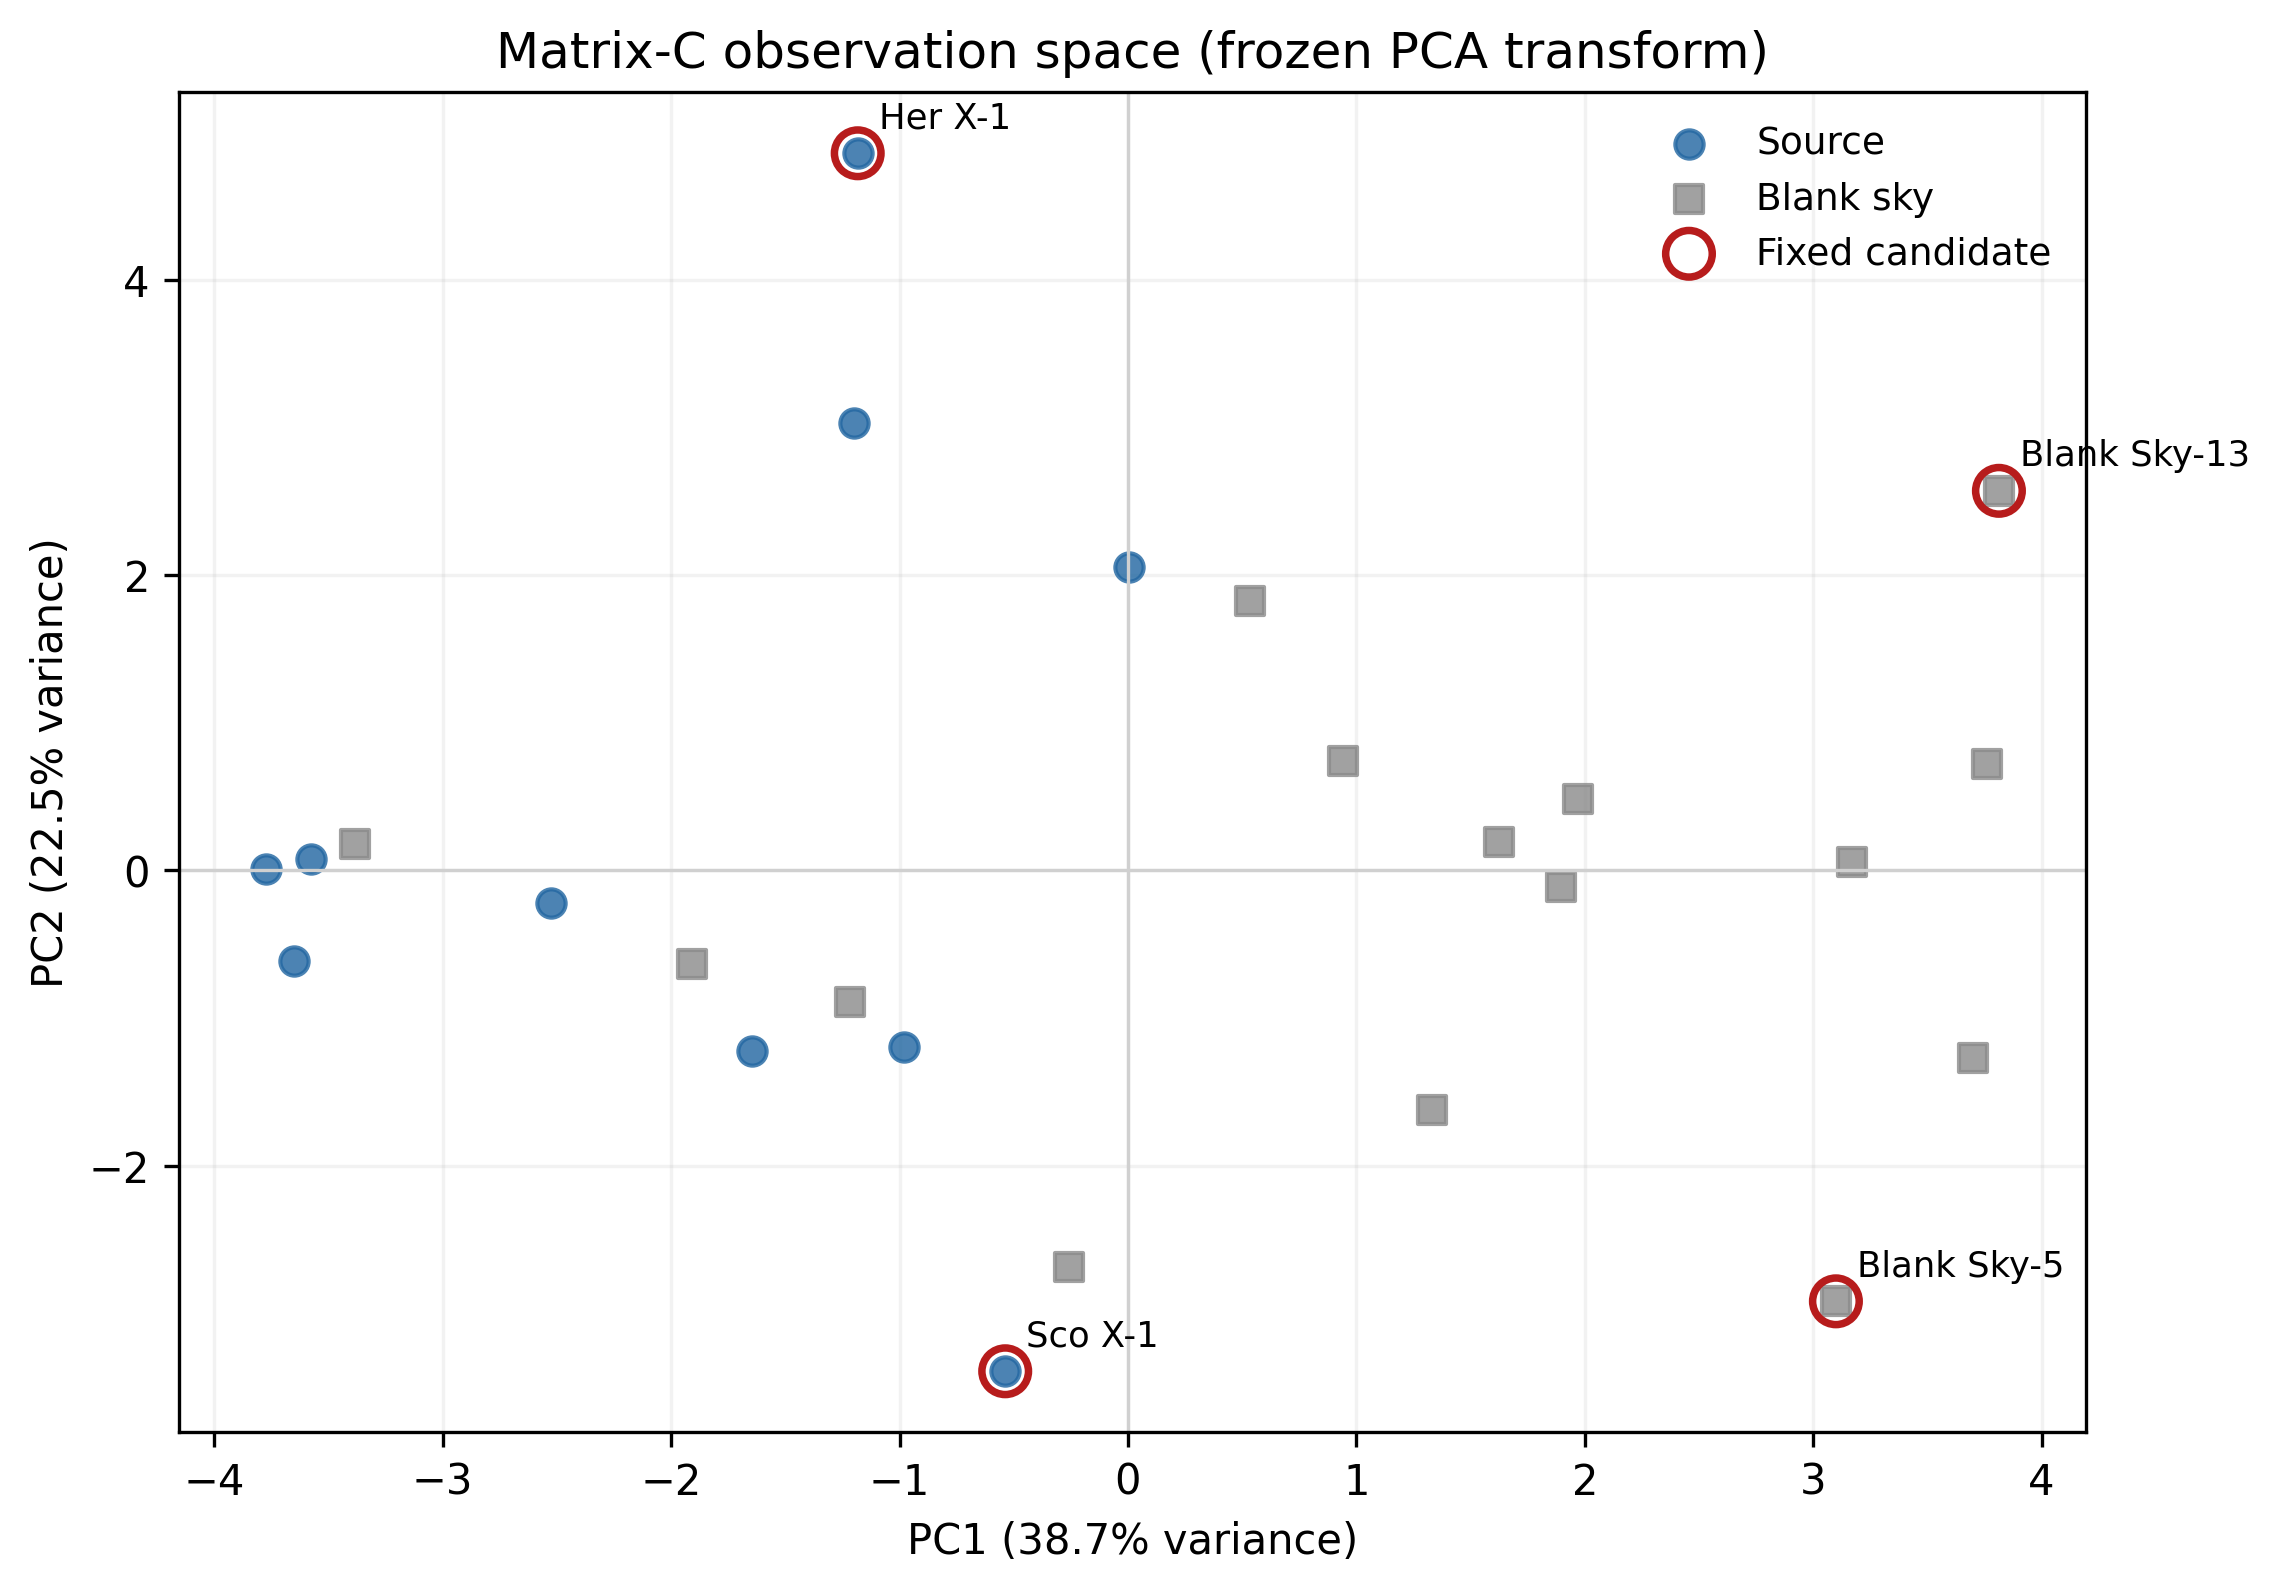
\includegraphics[width=\columnwidth]{fig2_matrix_c_pca.png}
\caption{Saved Matrix-C observations projected with the saved scaler and PCA transform. Fixed candidates are distinguished from other observations.}
\label{fig:pca}
\end{figure}

\section{Explainable Unsupervised Methodology}
\subsection{Saved Screening Pipeline}
For observation vector $\mathbf{x}_i$, the saved StandardScaler produces $\mathbf{z}_i$. PCA projects standardized observations into two components. KMeans uses $k=5$, \texttt{n\_init=20}, and random state 42. Isolation Forest uses 100 trees, contamination 0.16, and random state 42. Its saved \texttt{predict} result alone defines the fixed Normal/candidate label. The anomaly score is not a probability, and contamination is an imposed screening assumption rather than an estimate of anomaly prevalence.

The components are complementary, not independent validators. Two KMeans clusters are singletons; Sco X-1 and Blank Sky-13 consequently have zero distance from their assigned centroids. Zero assigned-centroid distance does not imply that either is ordinary.

\subsection{Project-Specific Local Feature Ranking}
The explanation reports within-observation ranks from four terms:
\begin{align}
p_{ij}&=\sum_{r=1}^{2}|z_{ij}w_{rj}|\lambda_r,\\
k_{ij}&=(z_{ij}-c_{g(i)j})^2,\\
o_{ij}&=s(\mathbf{z}_i)-s(\mathbf{z}_i^{(j\leftarrow0)}),\\
a_{ij}&=|z_{ij}|.
\end{align}
Each feature-wise term is normalized by its maximum absolute value within the observation, and only positive occlusion deltas enter:
\begin{equation}
e_{ij}=N(p_{ij})+N(k_{ij})+N(\max(o_{ij},0))+N(a_{ij}).
\end{equation}
The score measures composite model-informed local evidence under project choices. It does not decompose the Isolation Forest label, provide causal attribution, or support comparison of absolute importance between observations. Product mappings and explanation sentences are deterministic Python outputs; no large language model generates them.

\subsection{Feature-Neutralization Sanity Check}
The exploratory explanation analysis contains six cases and is distinct from the fixed four. High-ranked standardized features are set to zero, after which PCA distance and Isolation Forest score are recomputed. The project calls reductions in both Strong and a partial response Moderate. The saved reproduction gives five Strong, one Moderate, and zero Weak verdicts. KMeans is absent from this verdict. This is a six-case in-sample sanity check, not statistical, causal, or external validation.

\section{Independent Harmonic Diagnostic}
WeightedRoll is exposure-weighted and contains source and background contributions \cite{polix_handbook_2025}. For roll-bin centre $\phi$, Notebook 11 fits
\begin{equation}
y(\phi)=C+Q\cos(2\phi)+U\sin(2\phi)
\end{equation}
by inverse-variance weighted linear least squares. Fractional coordinates are $q=Q/C$ and $u=U/C$, with
\begin{equation}
m_{\mathrm{raw}}=\frac{\sqrt{Q^2+U^2}}{C},\qquad
\psi_{\mathrm{fit}}=\frac{1}{2}\operatorname{atan2}(U,Q).
\end{equation}
The coefficients are not calibrated sky Stokes parameters; raw modulation is not polarization degree (PD), and fitted phase is not official sky polarization angle (PA).

Fits with reduced chi-square $\chi_\nu^2\le2$ are classified acceptable, $2<\chi_\nu^2\le5$ caution, and larger values poor. These study-specific bands are not p-values or detection thresholds. Thirteen of 15 blank-sky fits are acceptable. Their fractional coordinates define $\bar q=0.0090920$ and $\bar u=-0.0064782$, with sample standard deviations 0.0048569 and 0.0040190. The diagonal standardized distance is descriptive and ignores covariance, fit uncertainty, baseline-estimation uncertainty, and observation matching.

The manuscript uses the saved Notebook-11 CSV provenance. The later Flask service propagates raw-modulation uncertainty $A/C$ differently; the implementations are not combined. Detailed comparison belongs in supplementary material. No official background subtraction, official $\mu_{100}$, calibrated PD, or verified PA conversion is claimed.

\section{Results}
\subsection{Fixed Deployed Result}
The saved Matrix-C artifact reproduces 21 Normal outputs and four anomaly candidates: C24\_0018 (Blank Sky-13), G01\_0006 (Sco X-1), G01\_0003 (Her X-1), and C24\_0010 (Blank Sky-5). These labels mean statistically unusual within the project archive and require domain-expert inspection.

\subsection{Procedure-Qualified Stability}
In the existing 100-seed experiment, Blank Sky-13, Sco X-1, and Her X-1 were selected in 100/100 runs; Blank Sky-5 was selected in 29/100. Blank Sky-15, Normal under the fixed model, appeared in 68/100. The defensible summary is a ``three-candidate Matrix-C core stable under the tested procedures'' with a seed-sensitive threshold neighbourhood. It is not a general robust-anomaly claim. Contamination sensitivity varies thresholds over one ordering, and the jackknife is retrospective influence analysis rather than held-out validation; Sco X-1 was not selected by its held-out refit.

\begin{figure}[t]
\centering
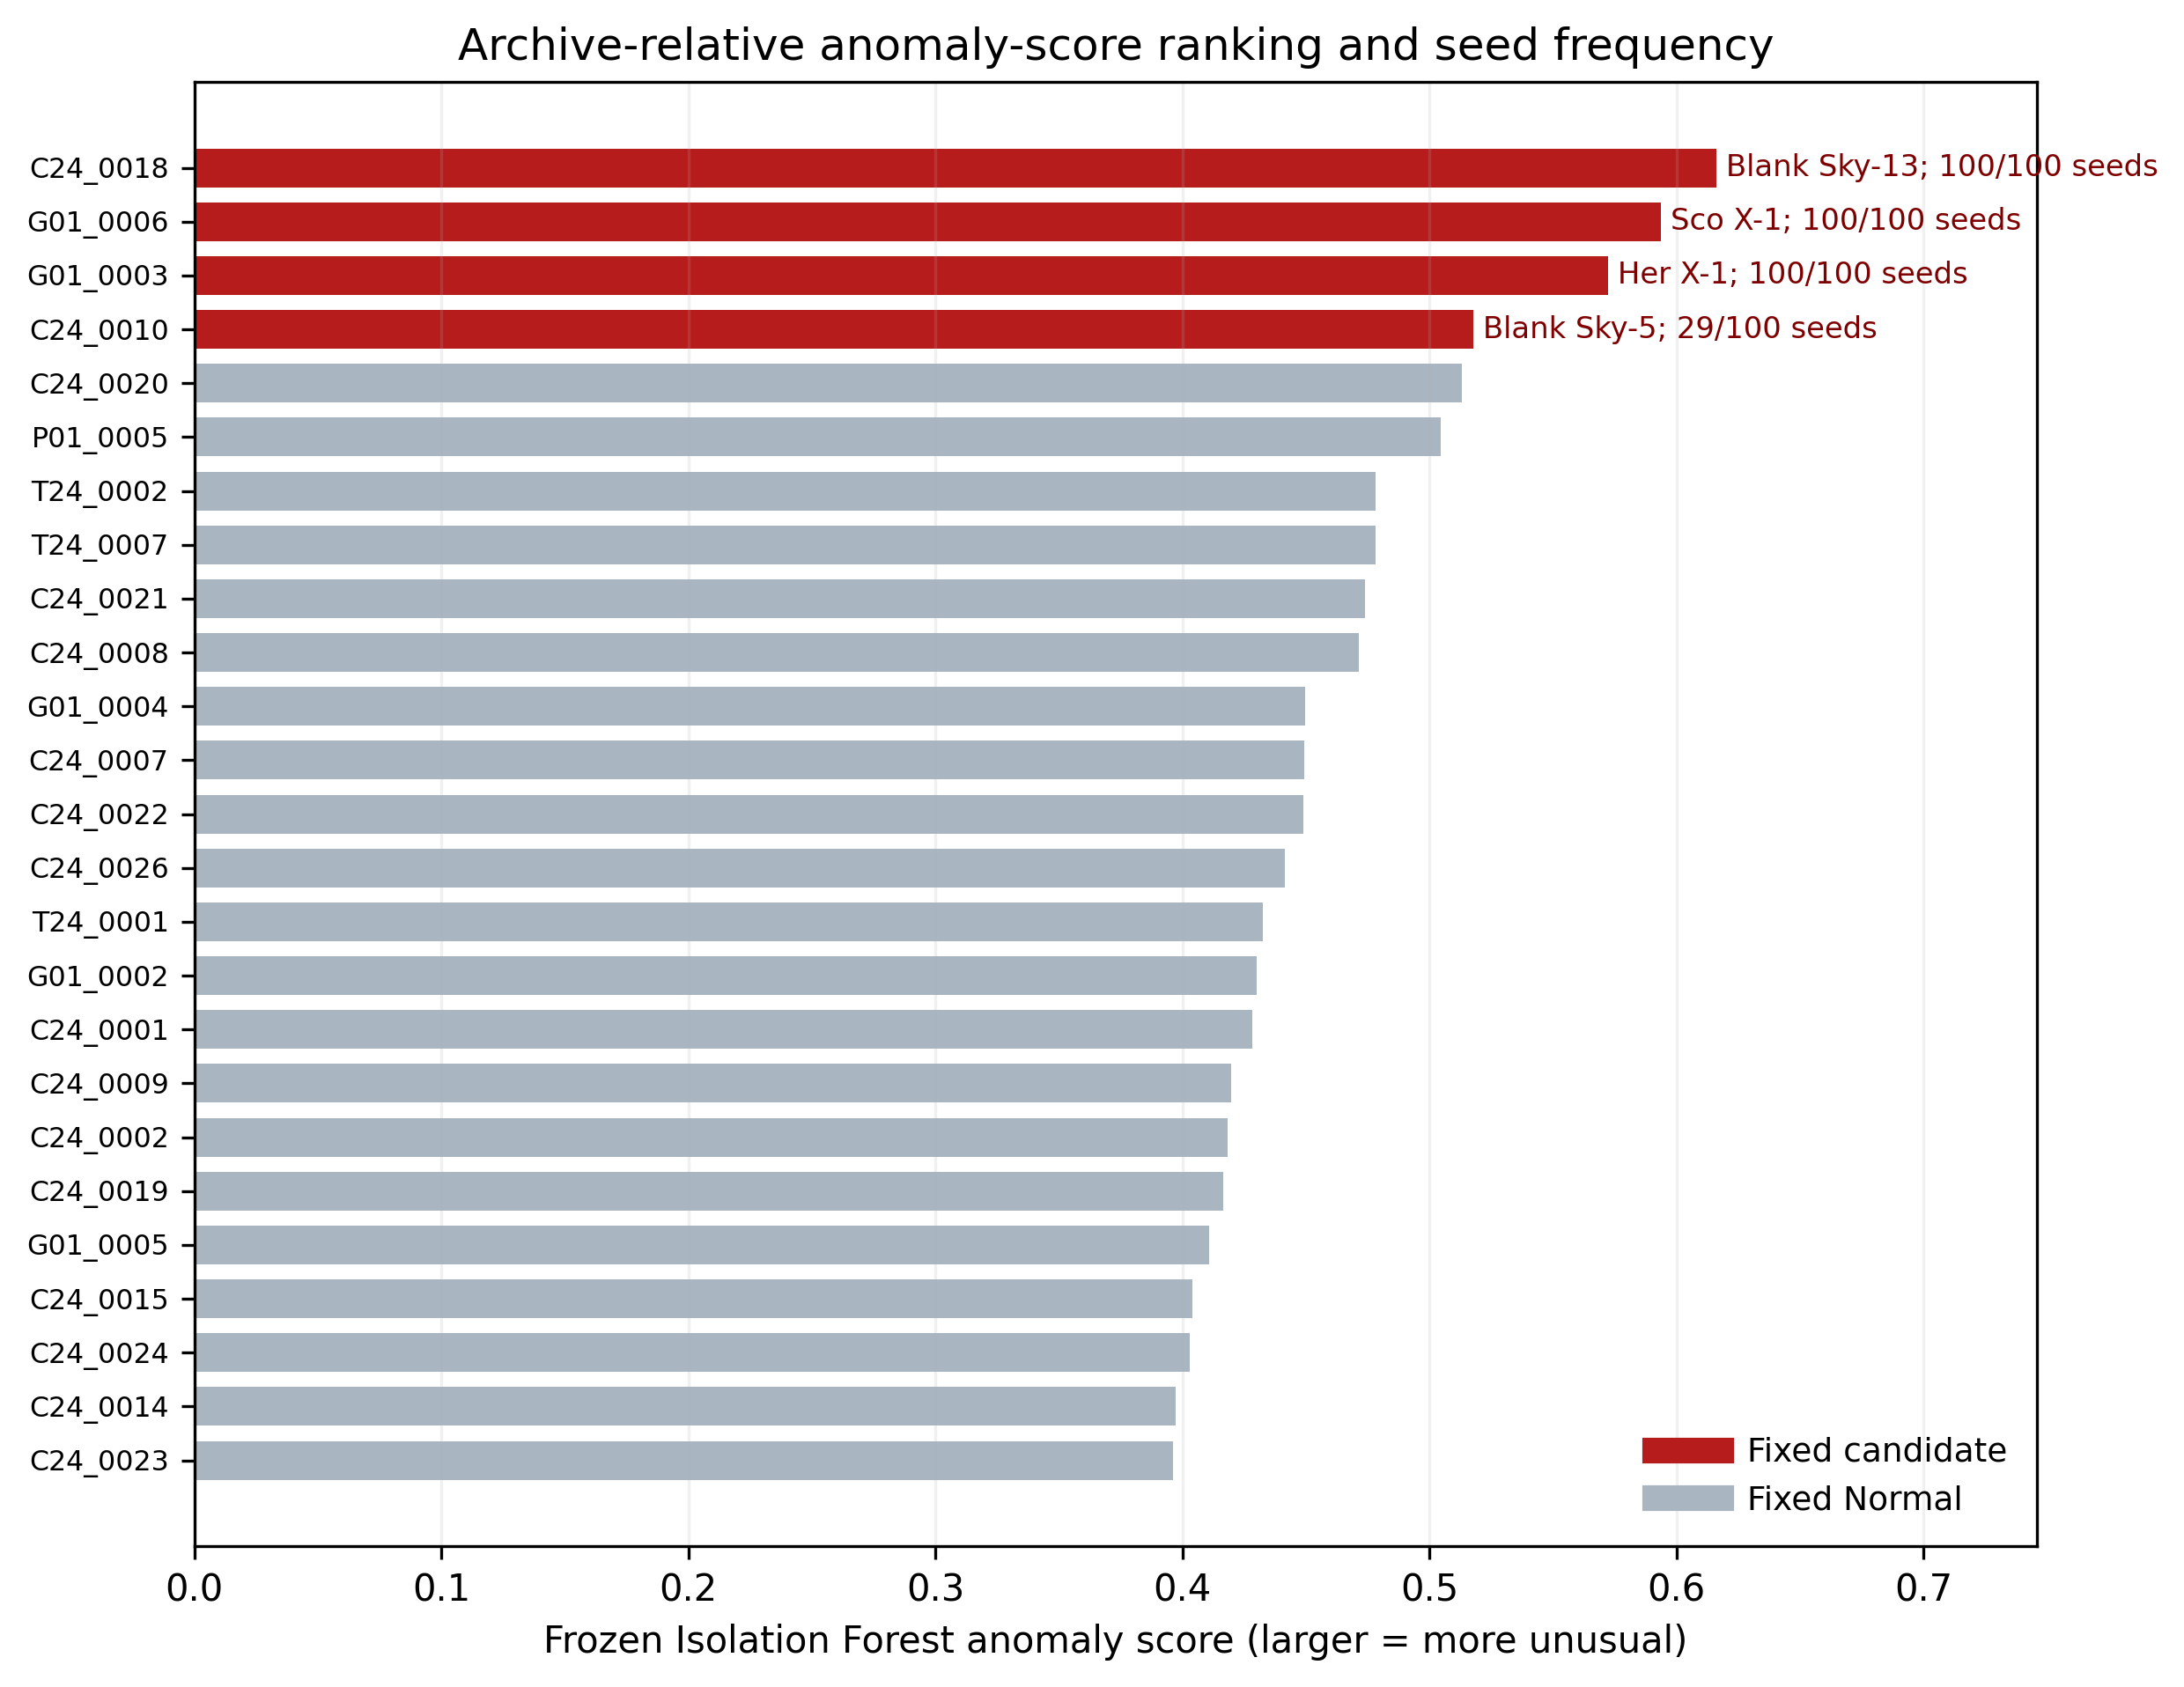
\includegraphics[width=\columnwidth]{fig3_fixed_candidate_ranking.png}
\caption{Saved Isolation Forest ranking with 100-seed selection frequencies. Candidate status follows the saved model.}
\label{fig:ranking}
\end{figure}

\subsection{Cross-Feature-Tier Persistence}
Across Matrix A, B, and C candidate sets, Sco X-1 and Blank Sky-13 persist. Her X-1 appears only in Matrix C; Blank Sky-5 appears in B and C. This result is separate from the fixed four and the seed-stable three-case core. It shows representation dependence and does not establish Matrix-C superiority. WR is not counted as confirmation.

\subsection{Local Feature-Ranking Examples}
\begin{table*}[t]
\caption{Fixed Candidates, Stability, Feature-Tier Persistence, and Leading Local Evidence}
\label{tab:candidates}
\centering
\small
\begin{tabular}{lrrlp{6.2cm}}
\toprule
Observation & Fixed score & Seeds & A/B/C & Leading local evidence\\
\midrule
Blank Sky-13 (C24\_0018) & 0.615964 & 100/100 & A,B,C & Weighted channel spread (\texttt{t1A\_energy\_weighted\_std\_channel})\\
Sco X-1 (G01\_0006) & 0.593516 & 100/100 & A,B,C & Peak channel 2.454; weighted mean channel 2.207; entropy 1.814\\
Her X-1 (G01\_0003) & 0.572308 & 100/100 & C & Delivered-light-curve rate coefficient of variation\\
Blank Sky-5 (C24\_0010) & 0.517611 & 29/100 & B,C & Source-roll order-dependent roughness proxy\\
\bottomrule
\end{tabular}
\end{table*}

For Sco X-1, the versioned function ranks energy peak channel first, weighted mean channel second, and channel entropy third. A historical entropy-first narrative could not be reproduced from a located versioned artifact and is superseded. The ranks do not identify an astrophysical cause or calibrated spectral property.

\subsection{Harmonic and Blank-Sky Results}
All 25 WeightedRoll products have saved fits: 19 acceptable, three caution, and three poor. The 13 qualifying blank-sky fits have mean raw modulation 1.147820\% and sample standard deviation 0.565960\%. All ten source values fall within the declared empirical mean $\pm2$ sample-standard-deviation scalar range. This is not a polarization-detection criterion.

\begin{table*}[t]
\caption{Representative Harmonic and Blank-Sky-Relative Results}
\label{tab:harmonic}
\centering
\small
\begin{tabular}{lrrrp{6.2cm}}
\toprule
Observation & Raw mod. (\%) & Category; $\chi_\nu^2$ & Distance & Bounded interpretation\\
\midrule
Sco X-1 (G01\_0006) & 1.1396 & Caution; 2.0308 & 0.3005 & Candidate; coordinates within the declared empirical blank-sky reference rule\\
Her X-1 (G01\_0003) & 0.5966 & Poor; 57.4335 & 2.3174 & Candidate; physical interpretation limited by poor fit\\
Crab (P01\_0005) & 1.6973 & Acceptable; 1.0625 & 1.2649 & Not fixed candidate; within declared scalar range\\
Blank Sky-13 (C24\_0018) & 0.8540 & Caution; 2.5658 & -- & Stable ML evidence does not imply acceptable fit\\
Blank Sky-5 (C24\_0010) & 1.5185 & Acceptable; 0.7134 & -- & Seed-sensitive ML flag coexists with acceptable fit\\
\bottomrule
\end{tabular}
\end{table*}
Uncertainties are omitted from the compressed table because the notebook/service propagation differs. Full central values, fit classes, and provenance remain in the supplementary plan.

\begin{figure}[t]
\centering
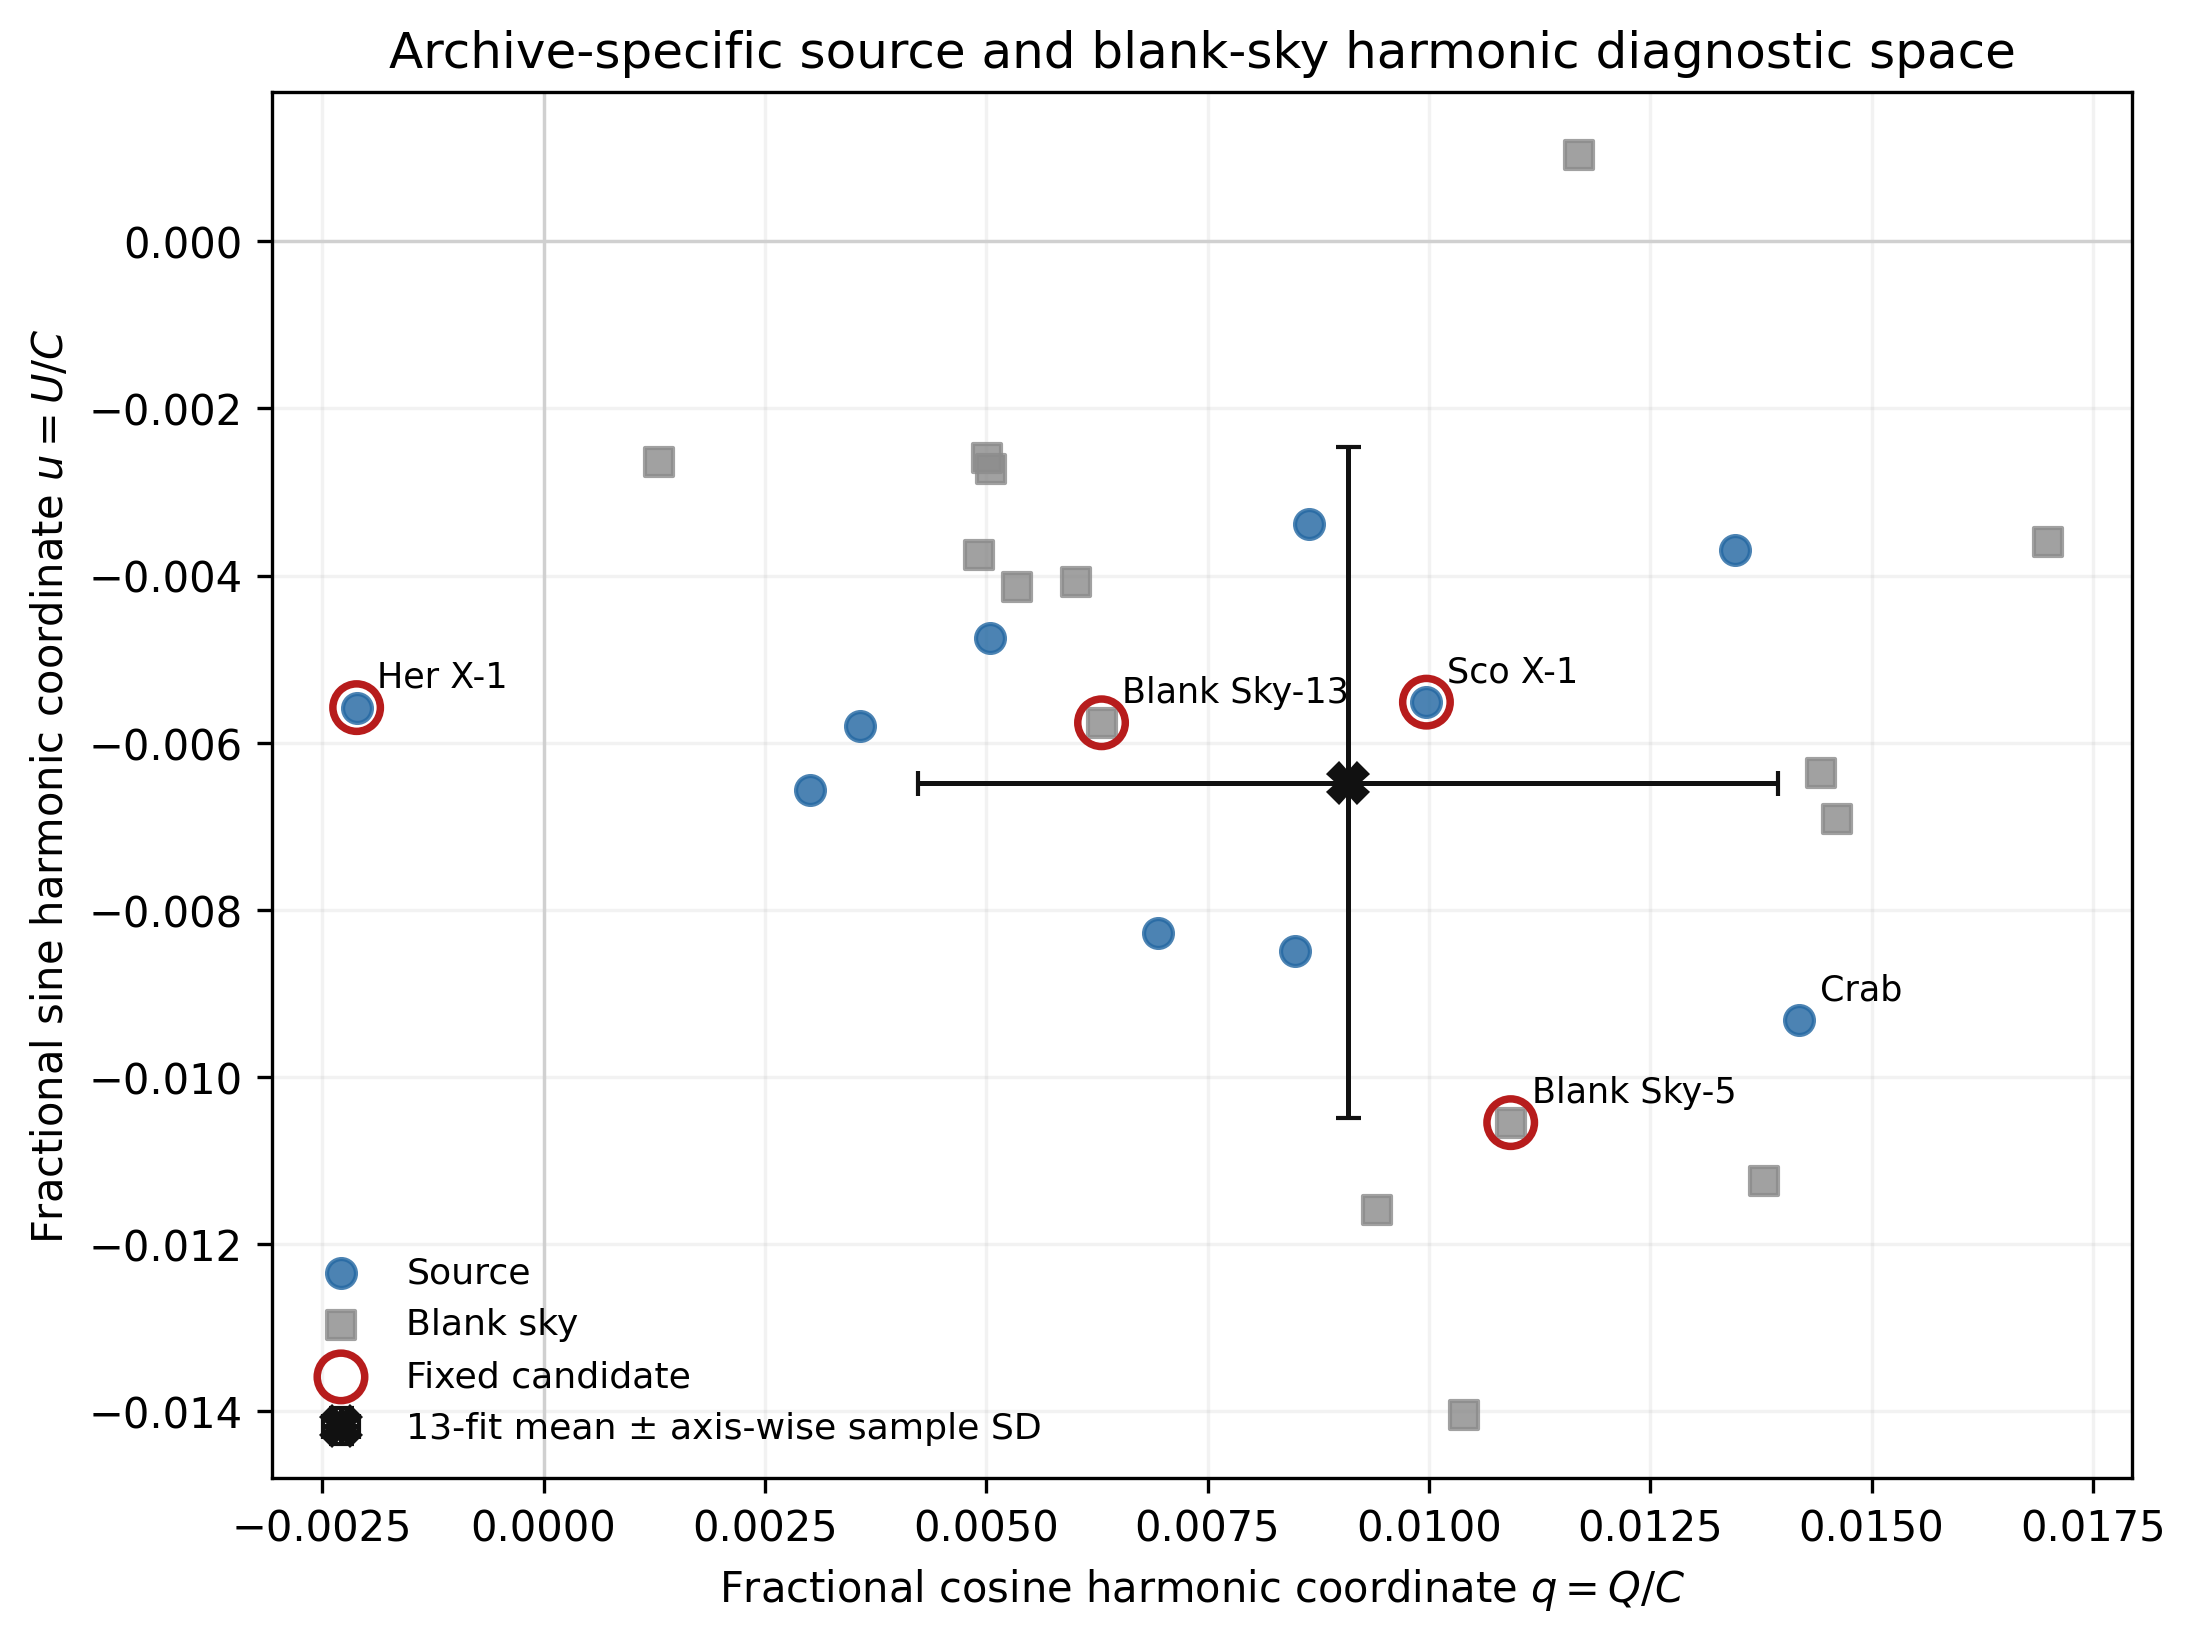
\includegraphics[width=\columnwidth]{fig4_fractional_harmonic_space.png}
\caption{Fractional harmonic coordinates from saved outputs. The empirical centre and coordinate distribution derive from 13 qualifying blank-sky fits; no confidence contour is implied.}
\label{fig:harmonic}
\end{figure}

\section{Discussion}
The main empirical finding is that statistical unusualness and modulation-like harmonic evidence are non-equivalent within the project archive. The branches do not measure the same property: Matrix C summarizes exposure, channel-distribution, source-azimuth, delivered-light-curve, and detector balance, whereas the physical branch summarizes source-plus-background roll modulation relative to an empirical blank-sky sample.

Sco X-1 is a fixed candidate and part of the seed-stable core. Its local ranking is dominated by channel-distribution proxies, while its harmonic coordinates lie near the empirical blank-sky centre. This supports inspection of its Level-2 channel products, not a polarization claim or spectral cause. Her X-1 is stable in Matrix C but not across A and B; its leading evidence is a delivered-light-curve proxy, and its simple harmonic fit is poor. The larger coordinate distance therefore has limited physical interpretation.

Crab P01\_0005 is not a fixed Matrix-C candidate, although its raw modulation is among the larger source values and its harmonic fit is acceptable. The value remains within the declared empirical blank-sky scalar range. Blank Sky-13 has strong screening stability but a caution fit; Blank Sky-5 has an acceptable fit but a seed-sensitive ML flag. No astrophysical or instrumental cause is assigned.

The framework's value is traceability. A researcher can move from a project-archive flag to named product-family summaries and separately inspect harmonic behaviour. This is a triage workflow, not an automated scientific decision system.

\section{Limitations and Threats to Validity}
The sample contains only 25 unlabeled observations, so accuracy and future-observation performance cannot be estimated. Scaling and models describe the same retrospective archive; the jackknife is not deployment validation. Contamination imposes the four-candidate threshold, feature-tier membership changes, and KMeans has singleton clusters.

Feature semantics are proxies: channel values are not calibrated energies, roughness depends on stored order, and delivered-light-curve features do not establish intrinsic variability. The XAI score is a within-observation heuristic with a six-case, in-sample neutralization check. WeightedRoll contains source and background; the selected 13-fit reference is not official subtraction, and the diagonal distance is not a confidence region. There is no official background procedure, official $\mu_{100}$, calibrated PD, or verified PA conversion.

Notebook 11 and the later service propagate raw-modulation uncertainty differently. The saved artifact was also audited under a scikit-learn version different from the artifact record, and the original environment was not fully pinned. Feature semantics and representative physical interpretation need POLIX-aware review. The Flask interface is a proof of concept without future-release drift validation.

\section{Conclusion}
This work implemented a traceable framework that compresses heterogeneous POLIX Level-2 products into a 15-feature representation, applies a saved unsupervised screening stack, ranks local composite feature evidence, and keeps WeightedRoll harmonic analysis separate. In the 25 archived observations, the saved model produced 21 Normal outputs and four candidates. Three were stable across tested Isolation Forest seeds, while Blank Sky-5 was seed-sensitive.

Representative cases showed that Matrix-C unusualness and modulation-like harmonic behaviour do not identify the same property within this archive. The framework supports researcher triage and product-level inspection; it does not establish astrophysical anomalies, polarization, calibrated PD, or official sky polarization angle. Future use should incorporate new releases, official background and calibration information, a pinned environment, and prospective expert-reviewed validation.

\section*{Acknowledgment}
The acknowledgment wording follows the current ISSDC guidance \cite{issdc_xposat_ack}.

This publication uses the data from the XPoSat mission of the Indian Space Research Organisation (ISRO), archived at the Indian Space Science Data Centre (ISSDC).

\bibliographystyle{IEEEtran}
\bibliography{03_FINAL_REFERENCES}
\end{document}
